\begin{figure}[h]
\centering
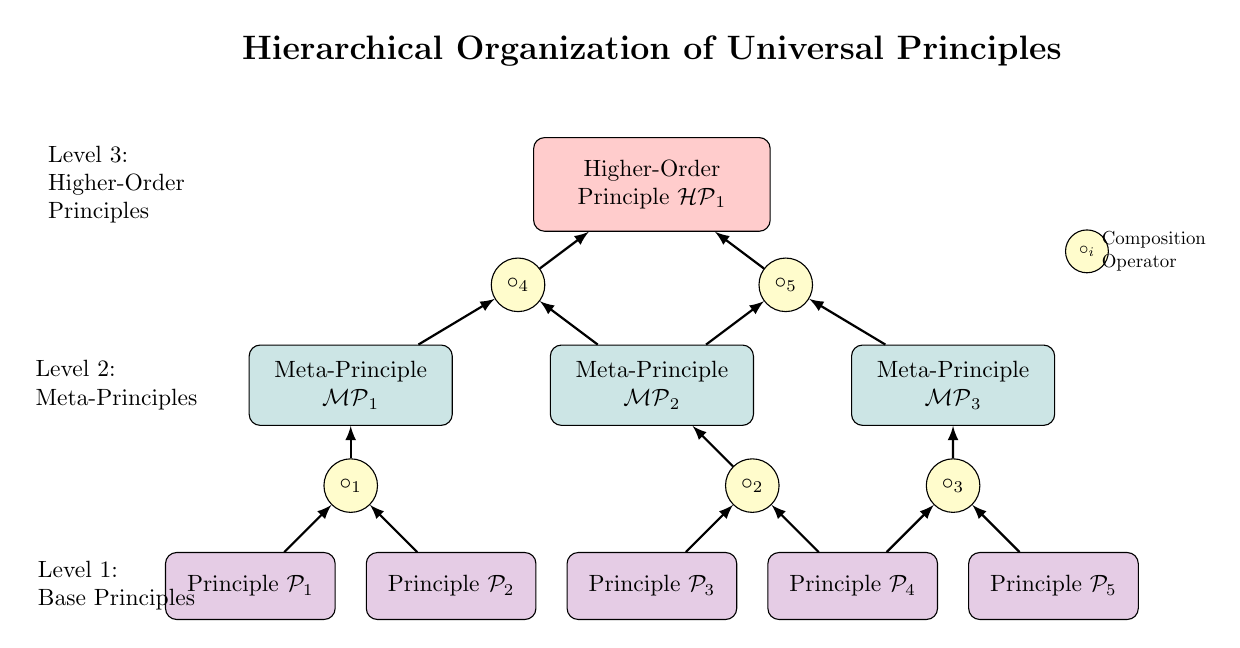
\begin{tikzpicture}[scale=0.85, transform shape]
    % Define styles
    \tikzstyle{principle} = [draw, fill=violet!20, rounded corners, minimum width=2.5cm, minimum height=1cm, text width=2.3cm, align=center]
    \tikzstyle{metaprinciple} = [draw, fill=teal!20, rounded corners, minimum width=3cm, minimum height=1.2cm, text width=2.8cm, align=center]
    \tikzstyle{highprinciple} = [draw, fill=red!20, rounded corners, minimum width=3.5cm, minimum height=1.4cm, text width=3.3cm, align=center]
    \tikzstyle{arrow} = [->, >=latex, thick]
    \tikzstyle{composition} = [circle, draw, fill=yellow!20, minimum size=0.8cm, align=center]
    
    % Base principles (level 1)
    \node[principle] (p1) at (0,0) {Principle $\mathcal{P}_1$};
    \node[principle] (p2) at (3,0) {Principle $\mathcal{P}_2$};
    \node[principle] (p3) at (6,0) {Principle $\mathcal{P}_3$};
    \node[principle] (p4) at (9,0) {Principle $\mathcal{P}_4$};
    \node[principle] (p5) at (12,0) {Principle $\mathcal{P}_5$};
    
    % Meta-principles (level 2)
    \node[metaprinciple] (mp1) at (1.5,3) {Meta-Principle $\mathcal{MP}_1$};
    \node[metaprinciple] (mp2) at (6,3) {Meta-Principle $\mathcal{MP}_2$};
    \node[metaprinciple] (mp3) at (10.5,3) {Meta-Principle $\mathcal{MP}_3$};
    
    % Higher-order principle (level 3)
    \node[highprinciple] (hp1) at (6,6) {Higher-Order Principle $\mathcal{HP}_1$};
    
    % Composition operators
    \node[composition] (c1) at (1.5,1.5) {$\circ_1$};
    \node[composition] (c2) at (7.5,1.5) {$\circ_2$};
    \node[composition] (c3) at (10.5,1.5) {$\circ_3$};
    \node[composition] (c4) at (4,4.5) {$\circ_4$};
    \node[composition] (c5) at (8,4.5) {$\circ_5$};
    
    % Arrows from level 1 to composition operators
    \draw[arrow] (p1) -- (c1);
    \draw[arrow] (p2) -- (c1);
    \draw[arrow] (p3) -- (c2);
    \draw[arrow] (p4) -- (c2);
    \draw[arrow] (p4) -- (c3);
    \draw[arrow] (p5) -- (c3);
    
    % Arrows from composition operators to level 2
    \draw[arrow] (c1) -- (mp1);
    \draw[arrow] (c2) -- (mp2);
    \draw[arrow] (c3) -- (mp3);
    
    % Arrows from level 2 to composition operators
    \draw[arrow] (mp1) -- (c4);
    \draw[arrow] (mp2) -- (c4);
    \draw[arrow] (mp2) -- (c5);
    \draw[arrow] (mp3) -- (c5);
    
    % Arrows from composition operators to level 3
    \draw[arrow] (c4) -- (hp1);
    \draw[arrow] (c5) -- (hp1);
    
    % Level labels
    \node[align=left] at (-2,0) {Level 1:\\Base Principles};
    \node[align=left] at (-2,3) {Level 2:\\Meta-Principles};
    \node[align=left] at (-2,6) {Level 3:\\Higher-Order\\Principles};
    
    % Legend for composition operators
    \node[composition, scale=0.8] at (12.5,5) {$\circ_i$};
    \node[align=left, scale=0.8] at (13.5,5) {Composition\\Operator};
    
    % Title
    \node at (6,8) {\Large\textbf{Hierarchical Organization of Universal Principles}};
    
\end{tikzpicture}
\caption{The hierarchical organization of universal principles in the Elder system. Base principles combine through composition operators to form meta-principles, which in turn combine to form higher-order principles. This directed acyclic graph structure allows the Elder to represent complex knowledge relationships while maintaining mathematical tractability.}
\label{fig:hierarchical_principles}
\end{figure}